% Chapter Template

\chapter{Memristor Simulation} % Main chapter title

\label{Chapter5} % Change X to a consecutive number; for referencing this chapter elsewhere, use \ref{ChapterX}

\lhead{Chapter 5. \emph{Memristor Simulation}} % Change X to a consecutive number; this is for the header on each page - perhaps a shortened title

A numerical method for a memristor simulation was developed and tested in previous chapters based on drift-diffusion equations and finite difference. This chapter introduces the memristor's structure and physical parameters used for the simulation. It continues with a preliminary problem analysis to determine required mesh density and maximum possible time step. This preliminary analysis is followed by 1-D simulations of a memristor under various conditions.

\section{Memristor Structure}
%-Problem Analysis and assumptions, semiconductor vs memristor plots
Following figure (\ref{MemStc}) shows the structure of a simple memristor which will be taken as a basis for all the memristor simulations presented in this thesis. It consists of 2 metal contacts, a polymer conductor (PEDOT:PSS) and an electrolyte solution which has lithium and perchlorate ions (perchlorate/lithium density $\approx$ 6.02 $10^{23}$ $m^{-3}$). The memristor is about 1 cm long and 1 mm wide. The thickness of the conductive layer is around 1 $\mu$m. During experimentation the electrolyte is deposited on PEDOT via a syringe so its thickness can vary drastically but as long as the amount of ions in the electrolyte solution is enough to saturate PEDOT this does not make a significant difference in the operation of the memristor. For simulation it was assumed that there were always more than enough ions to saturate the PEDOT so the electrolyte was modeled as an infinite source/sink of ions. The top boundary of the electrolyte was assumed to be charge neutral at all times which provides a mechanism for moving ions in and out of the system. This way the movement of ions near the surface of the PEDOT can still be captured without having to simulate the ion movement for the entire electrolyte solution which is variable in size. 

\begin{figure}[!htp]
\centering
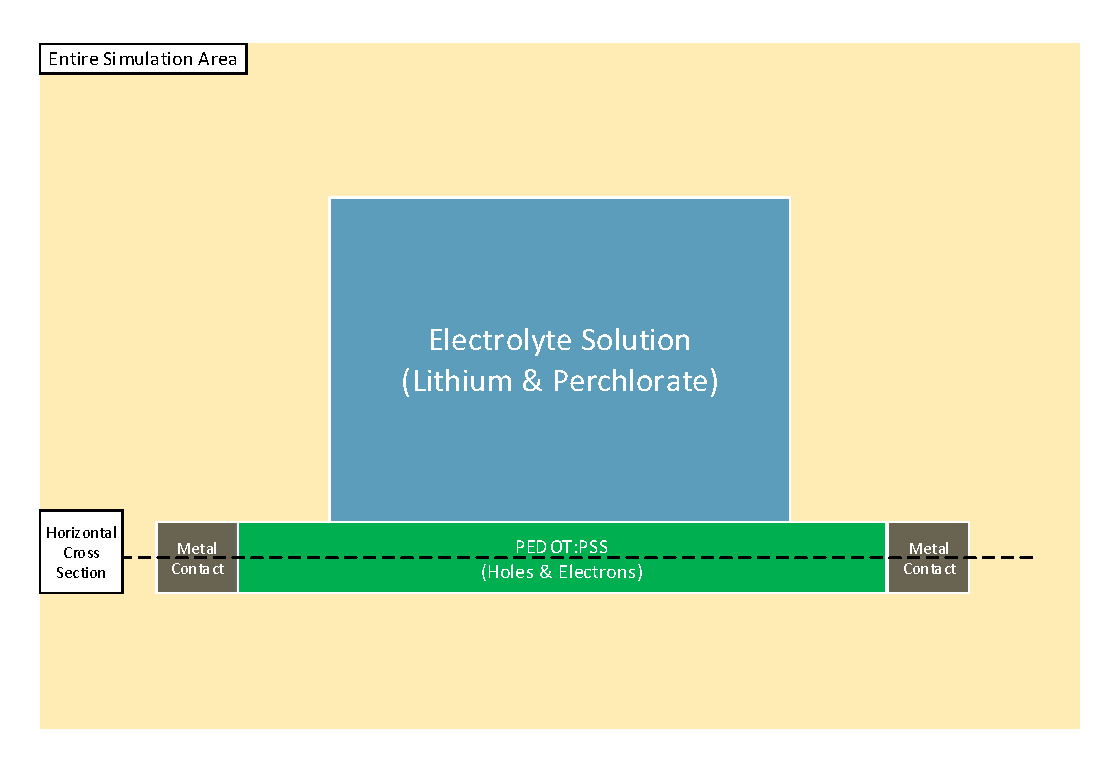
\includegraphics[scale=0.7]{Mem1}
\caption{} 
\label{MemStc}
\end{figure}

The initial conditions for all the charge carriers are the same. All charges are balanced and uniformly distributed but the carrier density in the electrolyte solution is higher than the carrier density in PEDOT. Perchlorate ions are not allowed to move outside the electrolyte solution so a no flow boundary condition was used around the electrolyte. Lithium ions are free to move between PEDOT and the electrolyte solution but their maximum concentration is limited inside the PEDOT. The mobility of lithium ions has further restrictions inside PEDOT. Lithium has higher mobility in PEDOT right under the electrolyte solution, wet PEDOT, than the region without any contact with electrolyte, dry PEDOT. In fact due to this difference very little amount of lithium reaches the metal contacts. This dec{rease in mobility was modeled by making the mobility of lithium a function of position. The mobility of lithium ions were assumed to be 100 times slower than the mobility of holes in the wet PEDOT and it is zero in the dry PEDOT( $\mu_{hole} \approx$ $10^{-3}$ $m^2/Vs$).  

PEDOT:PSS is a regular conductor with fixed negative charge and mobile holes. Holes can move in an out of the PEDOT through the metal contacts which hold the charge neutrality of the initial condition throughout the simulation. The interface between PEDOT and electrolyte only allows the exchange of lithium ions. During simulation,the movement of lithium ions changes the conductivity of the PEDOT by increasing or decreasing the amount of available holes through coulomb forces. In the actual device lithium ions change the conductivity via various physical effects like changing the mobility of holes through modifying their hopping distance. Even though the mobility of the holes can simply be made a function of time the physical details of these additional affects are beyond the scope of this thesis. 


\clearpage
\section{Simulation Requirements}

It is important to analyze computational requirements of a simulation in order to asses the feasibility of the computation scheme. In this case, it is possible to determine spacial and temporal requirements using the equations \ref{debye} to \ref{CFL_Drift} which describe physical and numerical limitations of the simulation. Following graph \ref{SpaceTime} shows the requirements for a memristor of the scale discussed above and a typical semiconductor device size around 1 $\mu$m. The mesh density has to be high enough in order to capture the exponential charge accumulation for charge shielding so the minimum step size was set to be 5 times smaller than the Debye length. Plots \ref{SpaceTime}.a and \ref{SpaceTime}.c show the amount of points required to simulate a semiconductor and a memristor based on minimum step size. It is important to note that these values are for 1-D simulation and they can be converted to 2-D and 3-D by squaring or cubing y axis values respectively. Plots \ref{SpaceTime}.b and \ref{SpaceTime}.d were created using CFL conditions for drift and diffusion and dielectric relaxation time. A typical simulation time was estimated using mobility and electric field. Based on the estimated simulation time the number of time steps were calculated using the minimum time step obtained from CFL conditions and dielectric relaxation time.

It can be seen from graphs \ref{SpaceTime}.a and \ref{SpaceTime}.c that memristor simulations require much higher mesh densities compared to a typical semiconductor simulation such as 1 $\mu$m long PN diode. This is due to the larger size and higher charge density of the memristor. Graph \ref{SpaceTime}.a \ref{SpaceTime}.b show that a memristor with $10^{26}$ $m^{-3}$ charge density of the electrolyte would require close to $10^9$ points and $10^{14}$ time steps to simulate in 1-D. These requirements make the simulation of the memristor extremely challenging. In order investigate and find possible solutions for this issue, first a memristor low charge density ($\approx 10^{15}$) was simulated in order to ensure that the simulation functions as designed. Then memristors with different charge densities were simulated and compared with each other to asses whether the behavior at low charge densities will be comparable to behavior at high charge densities.

\begin{landscape}
\begin{figure}[htp]
\centering
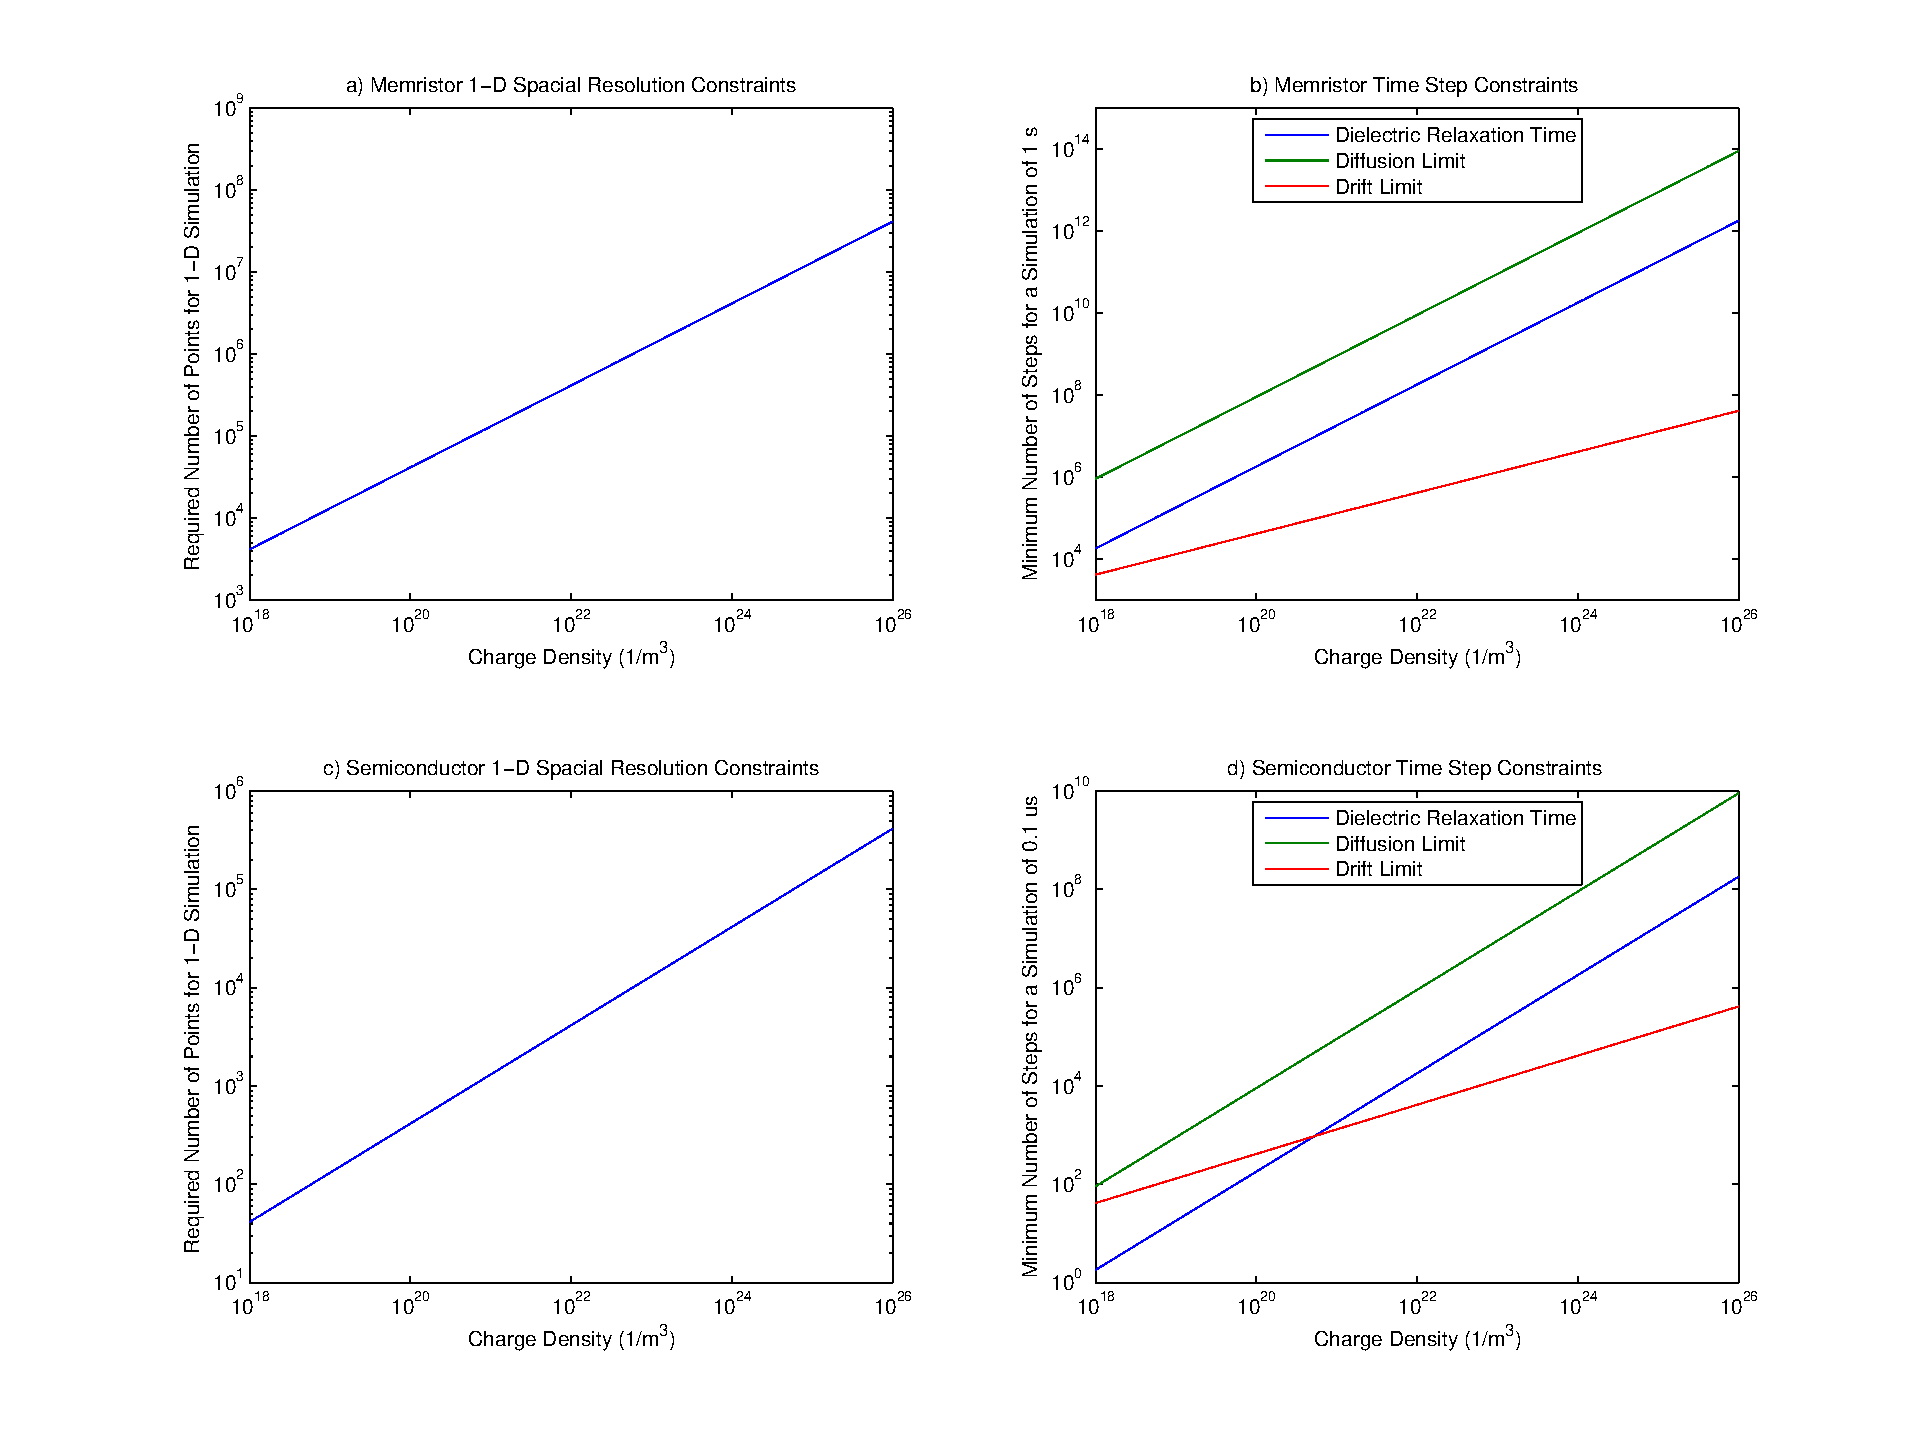
\includegraphics[scale=0.60]{SpaceTime}
\caption{Spatial and temporal requirements for simulation} 
\label{SpaceTime}
\end{figure}
\end{landscape}


\clearpage
\subsection{1-D Memristor Approximation}

The horizontal cross section from figure \ref{MemStc} has the most crucial elements of the memristor but its simulation in 1-D is not straight forward. This cross section through the PEDOT does not include the vertical movement of lithium. Without this effect, PEDOT is just a regular conductor with a uniform current density. In order to overcome this problem a generation/recombination term for lithium ions, calculated at every time step, was added to capture the vertical movement in addition to regular drift diffusion equations which represents the horizontal movement. This generation/recombination term can be symbolized as a current source with a resistor connected to all the nodes (figure \ref{MemStc15}). Perchlorate ions were not included in the simulation since they do not move into the PEDOT.

\begin{figure}[!htp]
\centering
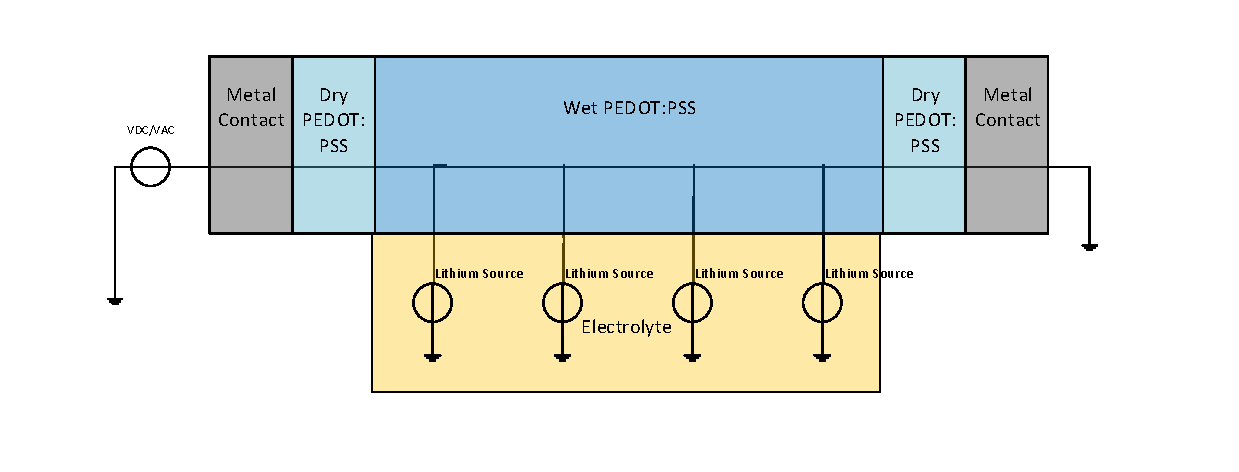
\includegraphics[scale=0.74]{1DMem}
\caption{1.5-D Memristor Structure} 
\label{MemStc15}
\end{figure}

The lithium source has two different terms, one for drift and another one for diffusion. It was assumed that the concentration of lithium was always constant in the electrolyte. This way the vertical diffusion current density can be calculated using the difference between the lithium density in PEDOT and electrolyte. For the diffusion term an electric field had to be estimated between the PEDOT and the electrolyte. First the potential of the electrolyte was assumed to be half of the net applied potential. Then an electric field was calculated using the electrolyte and the instantaneous potential of the PEDOT at different positions.

Since the main characteristic of memristor is the change in resistivity over time it is important to develop a standard approach for measuring it. For the simulations in this chapter and the following one, first all the simulations were run until steady state without the movement of lithium/perchlorate ions. Lithium and perchlorate ions start to move after the steady state has been reached. The movement of ions create another transient which includes changes in resistivity. The current density (at steady state) obtained from the initial simulation was used as a normalizing factor in order to determine the changes in resistivity after the ion movement has started.

\clearpage
\subsection{1-D Memristor Simulation Using a Pulse Train}
  
For the following simulation a potential pulse train, slow enough to let the memristor reach steady state, was applied on the left contact. Following plot \ref{MemResTrain} shows the resistivity measured using both contacts separately. As expected the resistance of the device more than doubled as the lithium ions move in. Additionally, it can be seen from the graph \ref{MemResTrain} that left and right contacts do not always show the same resistivity over the duration of the simulation. This is normal since the difference is due to PEDOT layer losing holes on one side which reduces the overall conductivity of the device. 

The resistivity in figure \ref{MemResTrain} shows a sudden drop when the potential is switched from 1 to 0 and vice versa. This sudden drop occurs because of the accumulation of lithium ions and holes near the negative contact which opposes the electric field generated due to the applied potential (see figure \ref{MemEss}). When the potential changes suddenly, previously opposing electric field now helps the movement of holes and lithium towards the other end of the device. This additional electric field momentarily reduces the resistivity of the device.

\begin{figure}[!htp]
\centering
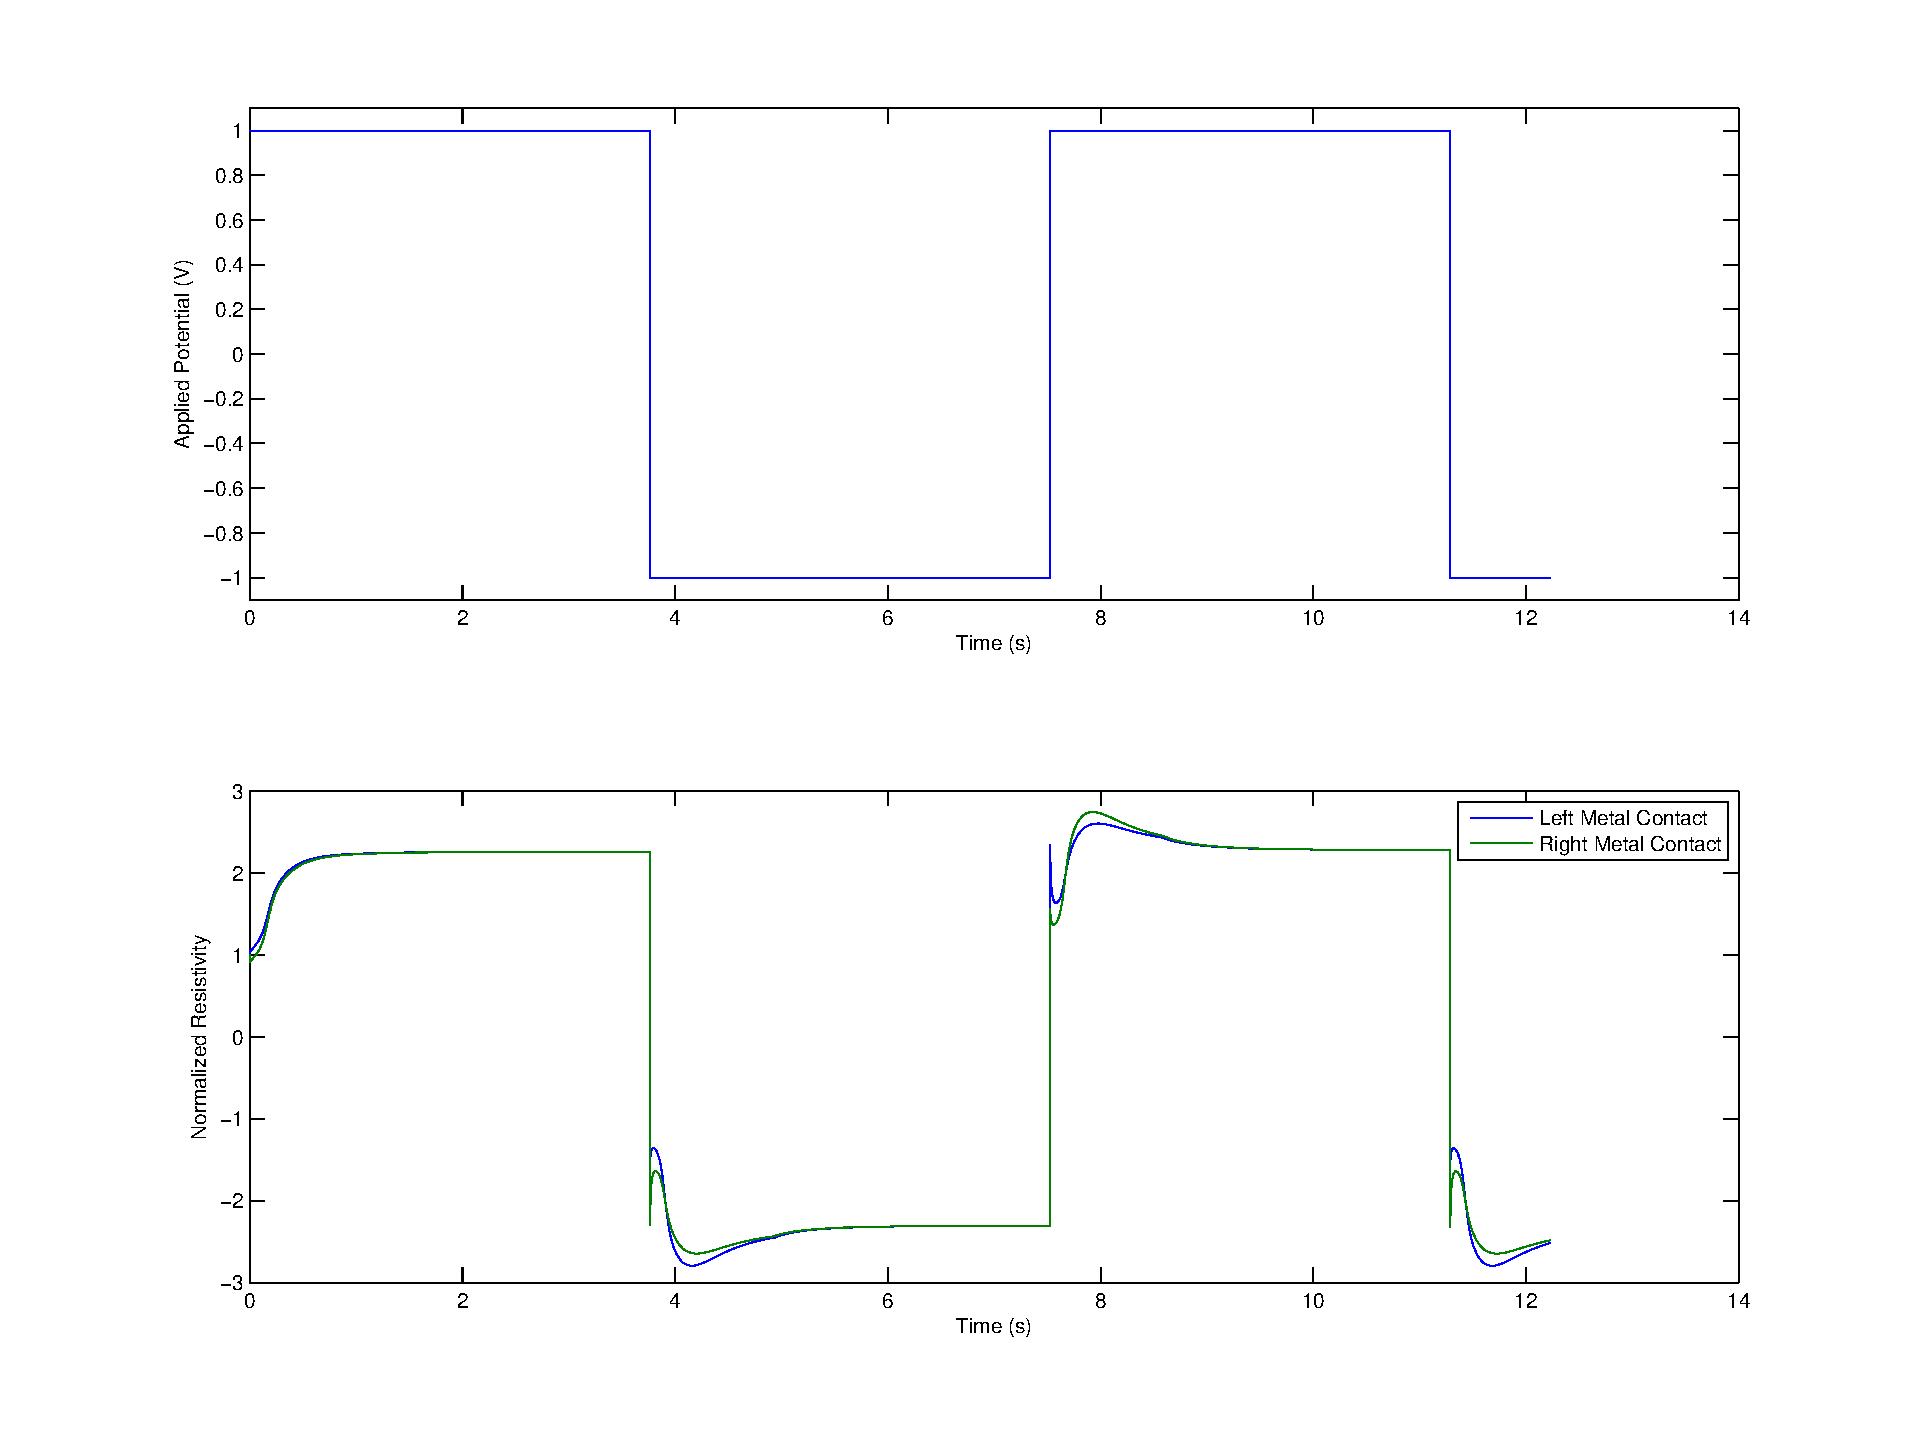
\includegraphics[scale=0.45]{1DMemPulseTrain}
%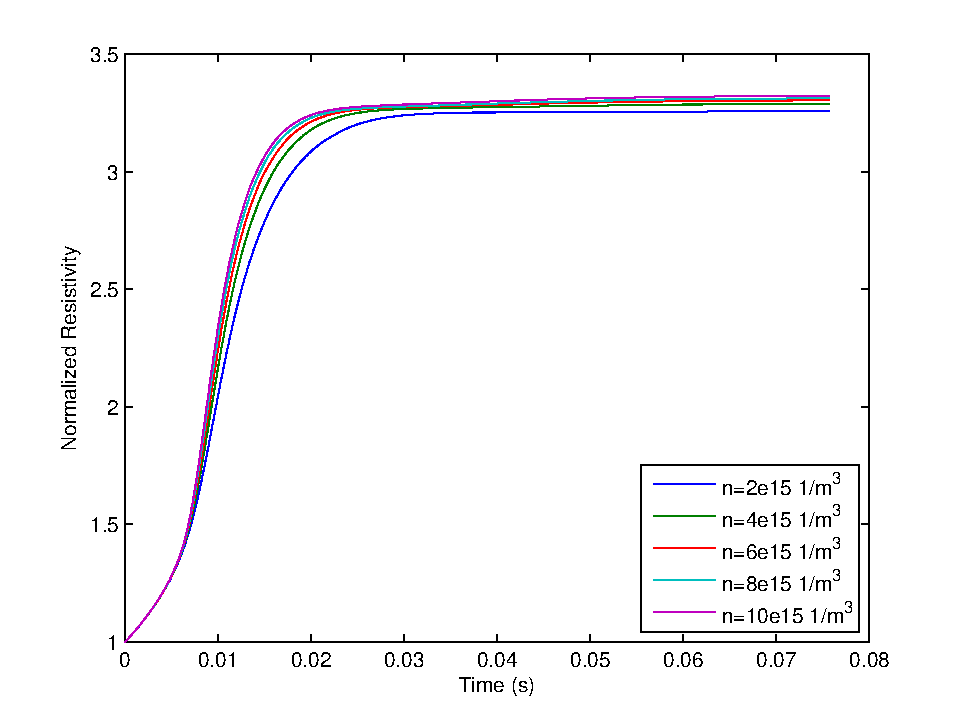
\includegraphics[scale=0.60]{Ex5DCResistivity}
\caption{Change in resistivity over time due to applied potential} 
\label{MemResTrain}
\end{figure}


\clearpage
Figure \ref{MempLi} demonstrates the replacement of holes by lithium ions over time which directly effects resistivity seen in figure \ref{MemResistivityTrain}.  As lithium ions get pulled in from the electrolyte toward the contact they accumulate inside PEDOT and push holes out via coulomb forces. Decreased hole concentration in the PEDOT increases the resistivity of the material. This change in resistivity over time is illustrated in figure \ref{MemResTrain}.

\begin{figure}[!htp]
\centering
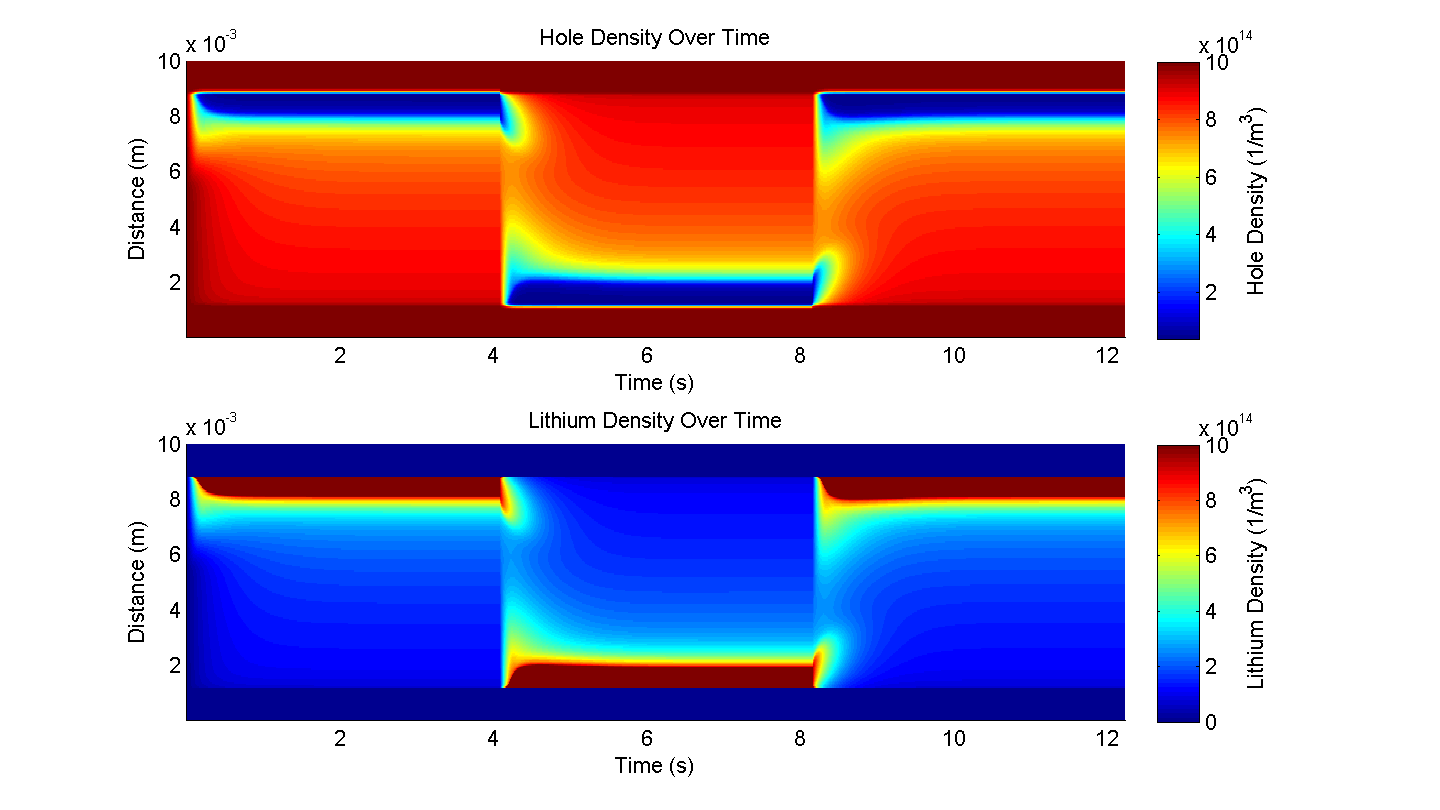
\includegraphics[scale=0.65]{1DMemDensityOverTime}
%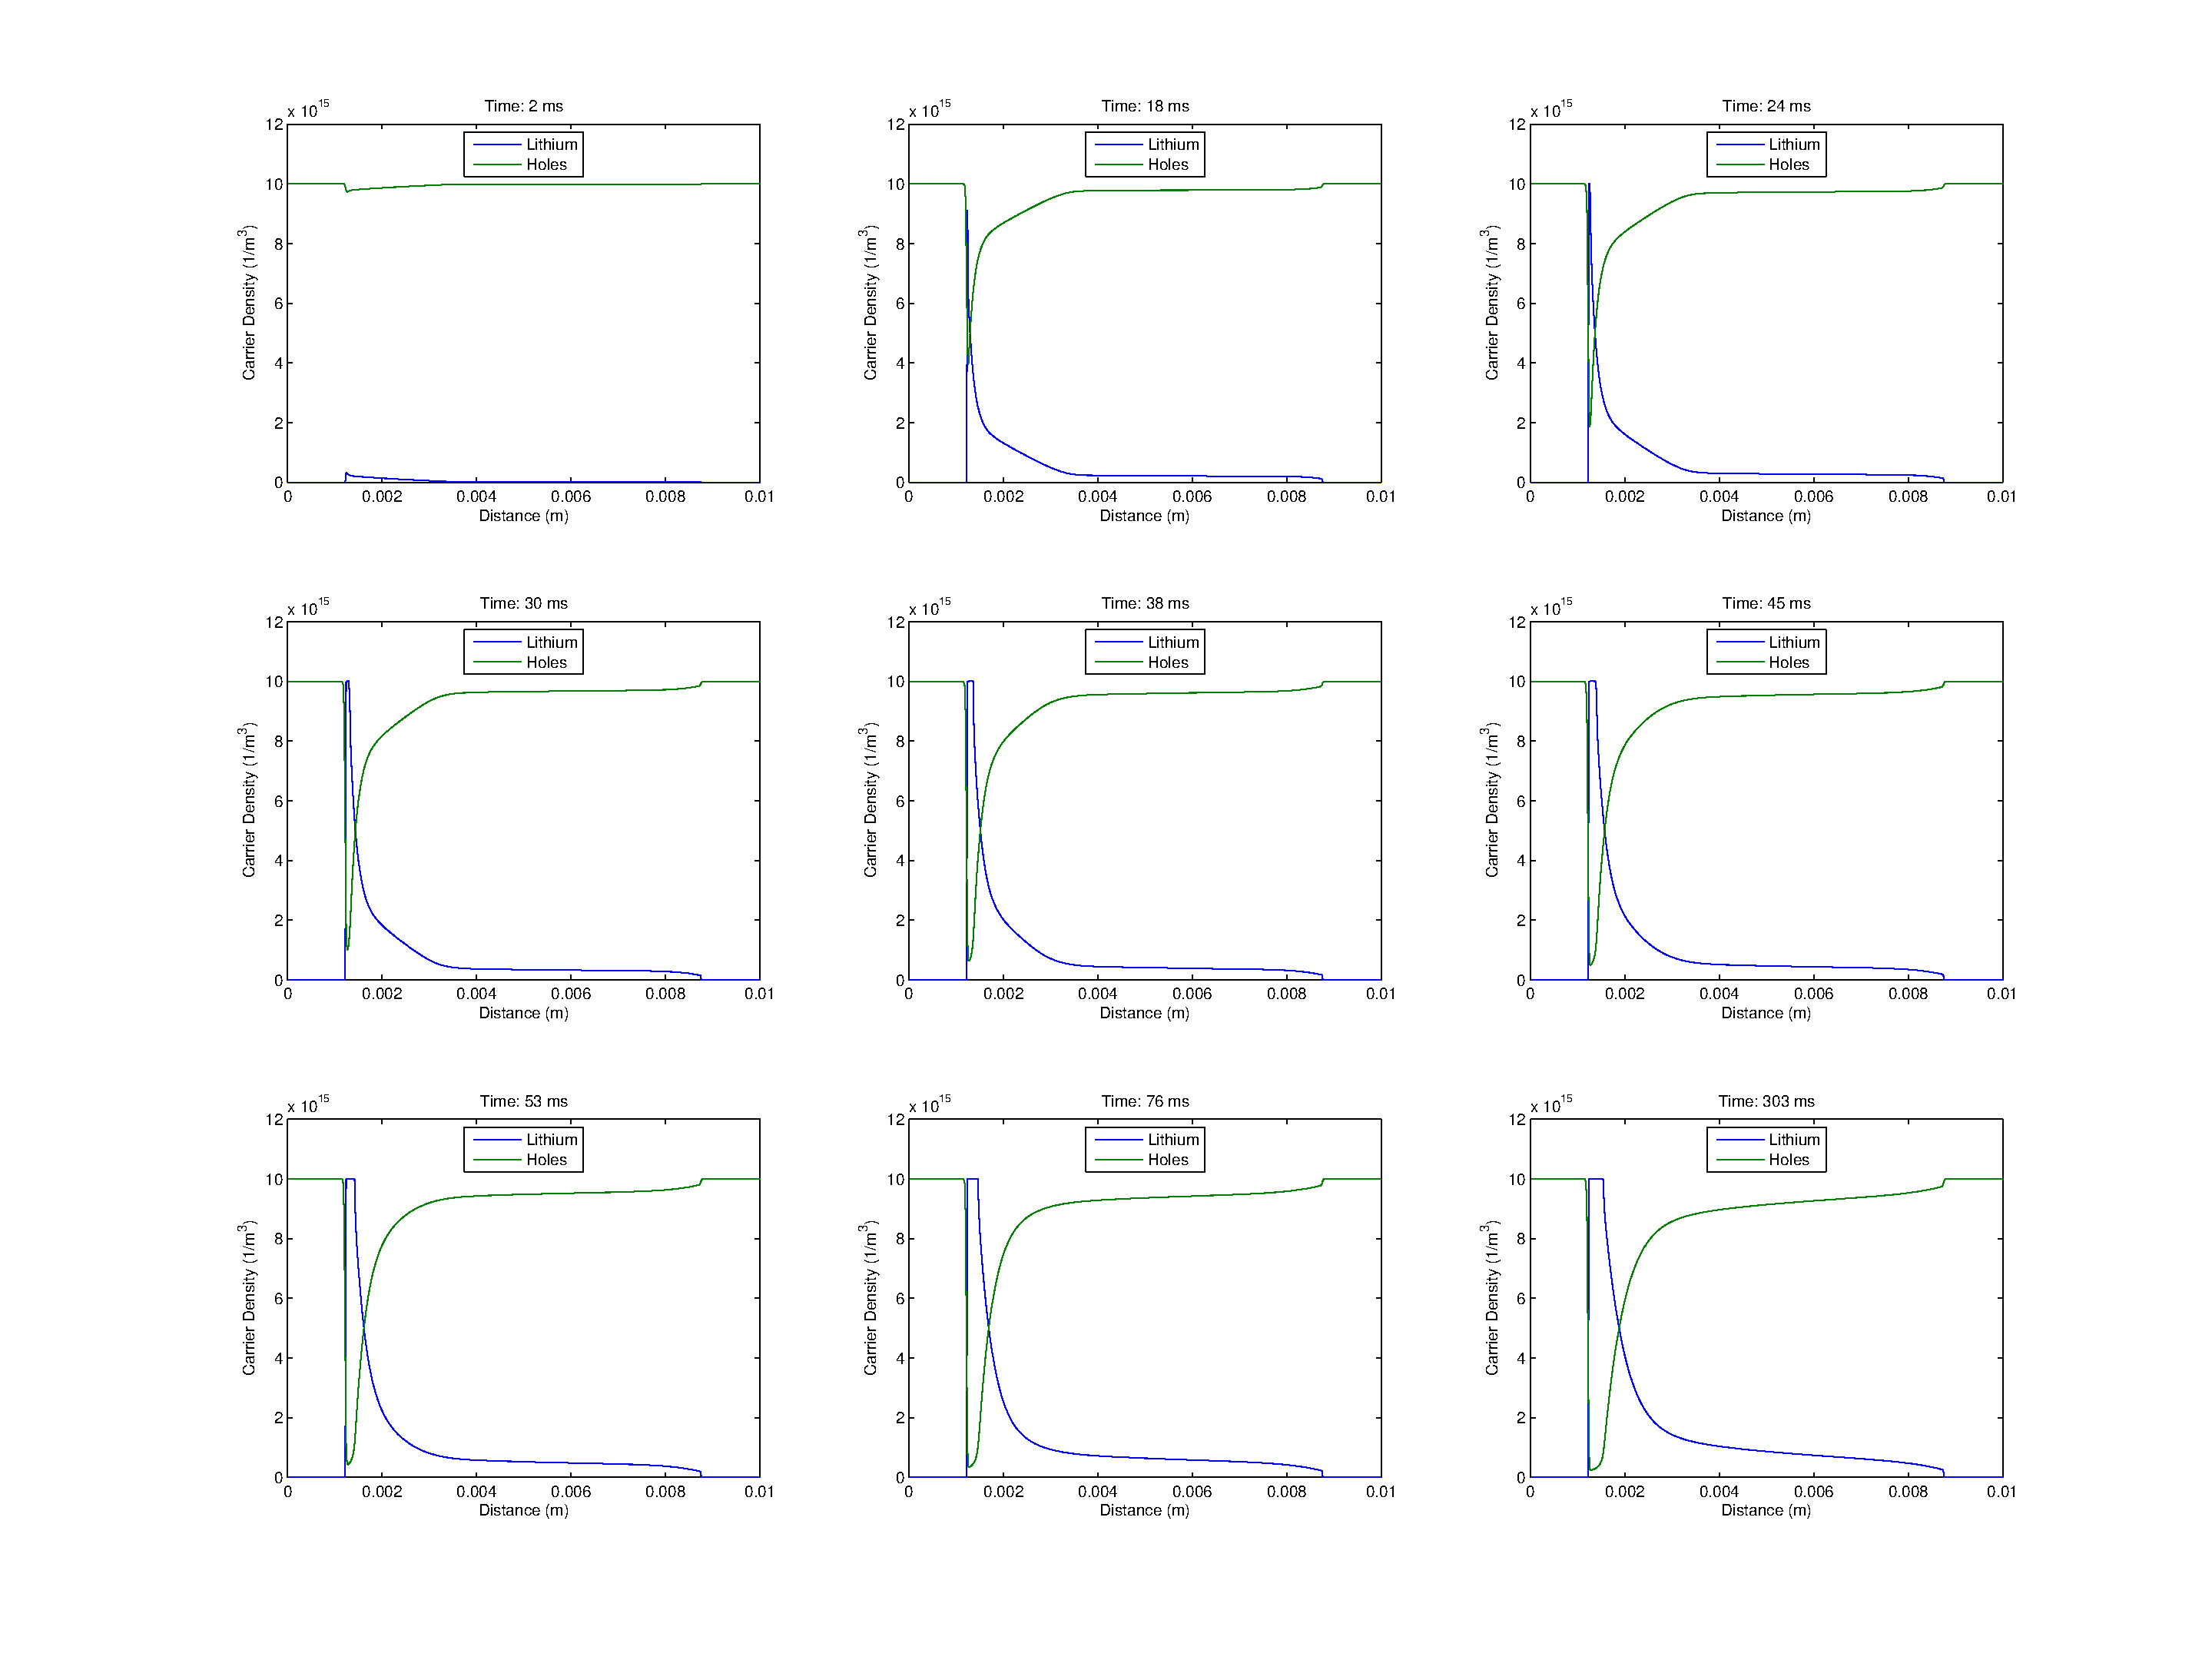
\includegraphics[scale=0.40]{Ex5pNp_Time1}
\caption{Lithium and hole density distribution over time} 
\label{MempLi}
\end{figure}

It is important to note that lithium ions are free to move in x and y direction. In figure \ref{MempLi} it can be seen that after the potential is switched as the lithium density moves from  side to the other. Most of the lithium movement happens through the exchange of ions between PEDOT and the electrolyte since the distance between them is far less than the length of the PEDOT. So the lithium ion, traveling from the positive to the negative contact, are pulled into the electrolyte before they reach the other side. Near the negative contact lithium ions are quickly pulled into the PEDOT and accumulate at the wet/dry interface. Figure \ref{MemResistivityTrain} shows the changes in resistivity throughout PEDOT due to the accumulation of lithium. The resistivity is increased in regions where there is high lithium accumulation. 

By examining the resistivity plot of PEDOT it is possible to conclude that it is composed of 3 distinct regions. 2 dry regions, where there is no contact with the electrolyte, have constant uniform resistance. Between these two resistances there is a variable non uniformly distributed resistance controlled by hole/lithium concentration and hole mobility. So this model captures the main characteristic of the memristor which is a variable resistance where the resistance at any time depends on the past of the device. Following equation gives the total resistance for the memristor model developed for this thesis:

\begin{equation}
\centering
R_{tot}=2R_{dry}+R(Li,p,\mu_{hole})
\end{equation}

The minimum resistance of this device is just the total resistance of the PEDOT without the lithium ions. The maximum resistance depends on different factors such as applied potential and the distribution and concentration of lithium ions inside PEDOT.

\begin{figure}[!htp]
\centering
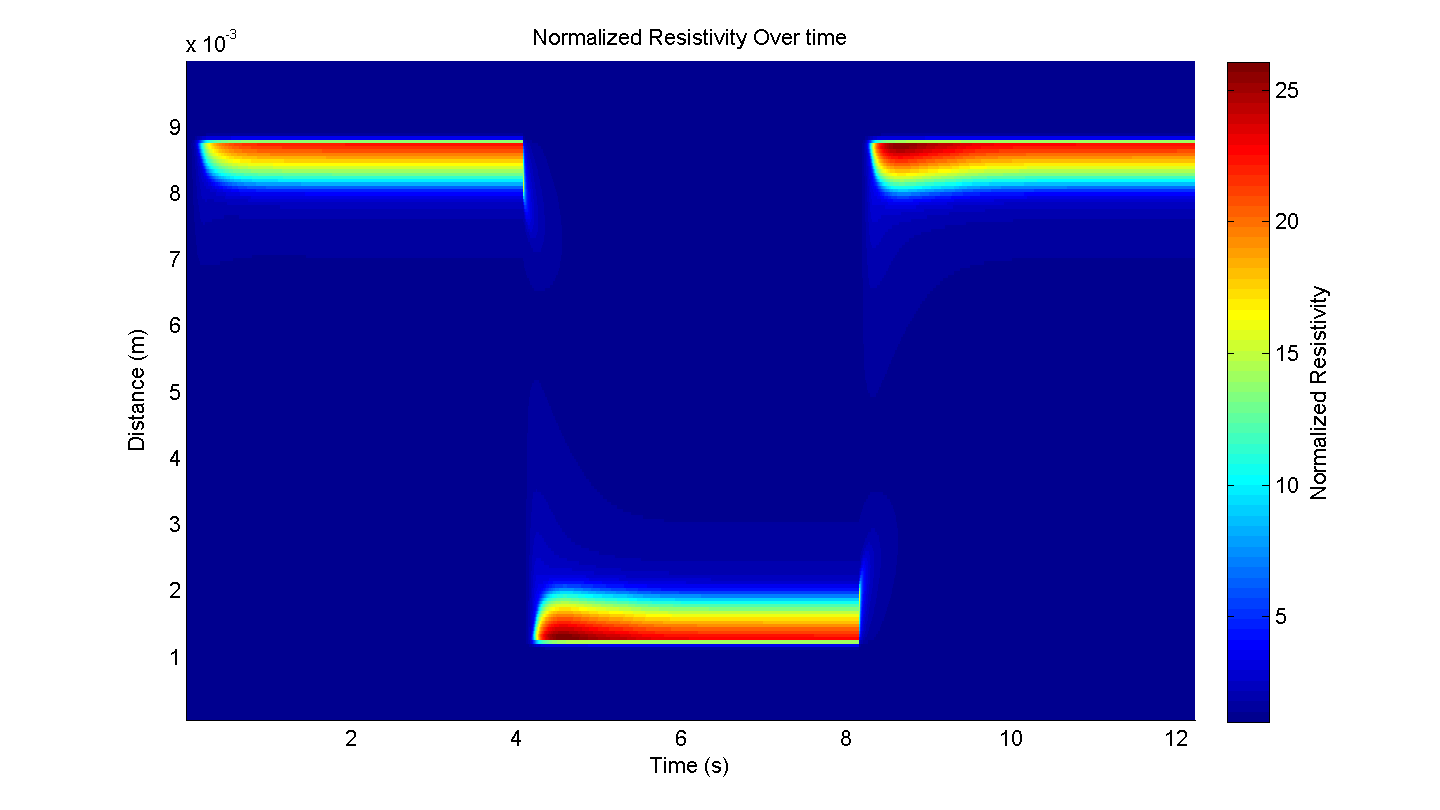
\includegraphics[scale=0.65]{1DMemResistivityOverTime}
\caption{Normalized resistivity over time} 
\label{MemResistivityTrain}
\end{figure}



\clearpage
(the following figures can go in appendix ?)


\begin{figure}[!htp]
\centering
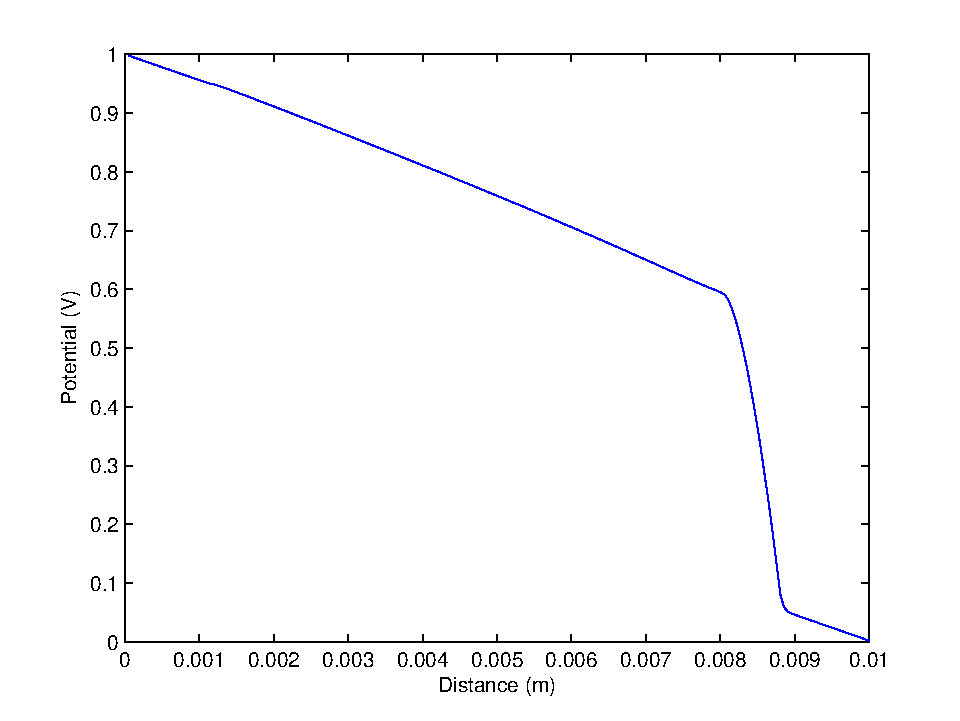
\includegraphics[scale=0.60]{1DMemPotentialSS}
\caption{Potential at steady state} 
\label{MemVss}
\end{figure}


\begin{figure}[!htp]
\centering
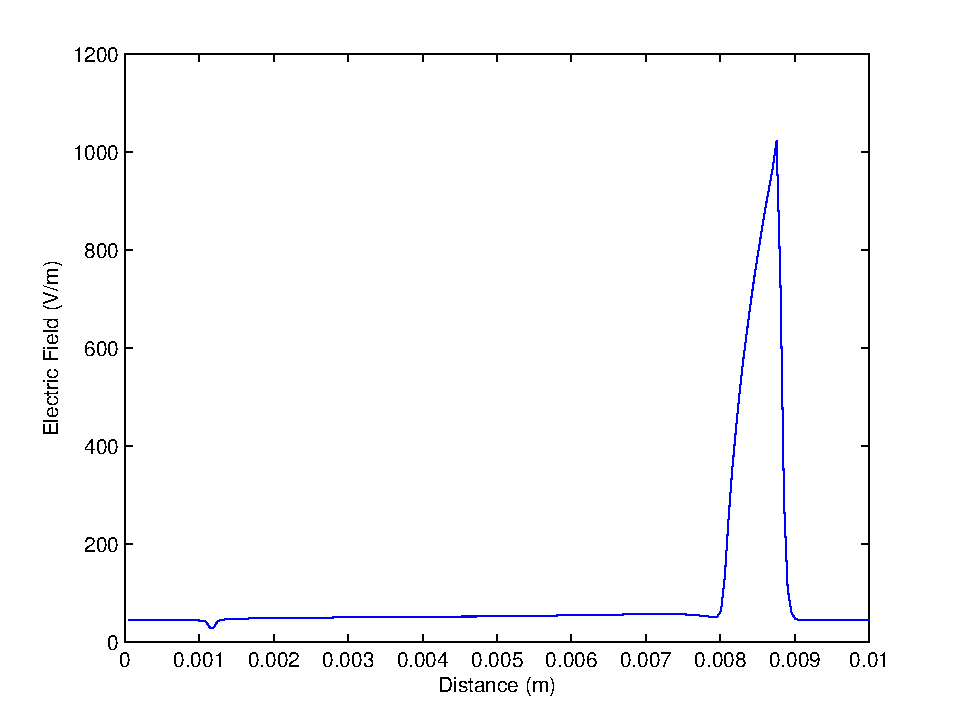
\includegraphics[scale=0.60]{1DMemEfieldSS}
\caption{Electric field at steady state} 
\label{MemEss}
\end{figure}



\clearpage
\subsection{1-D Memristor Simulation With Increasing Charge Density}

After establishing that the simulation behaves appropriately it is important to investigate how charge density effects this model since the size of the device limits the maximum charge density that can be simulated. The actual device has a hole density in the range of $ \approx 10^{22}$ $m^{-3}$ but the simulation is restricted to $\approx 10^{15}$ $m^{-3}$. Following 3 graphs (\ref{HoleDiff}, \ref{LithiumDiff} and \ref{DensityDiff} ) show hole and lithium densities as well as the current density at the right metal contact for various charge densities. The simulations were done on high mesh densities to allow stable simulation at high charge concentrations. All the values were normalized to the initial plot using respective hole/lithium density ratios.


\begin{equation}
\centering
n_i= n_i * Dn_i/Dn_1
\end{equation}


\begin{figure}[!htp]
\centering
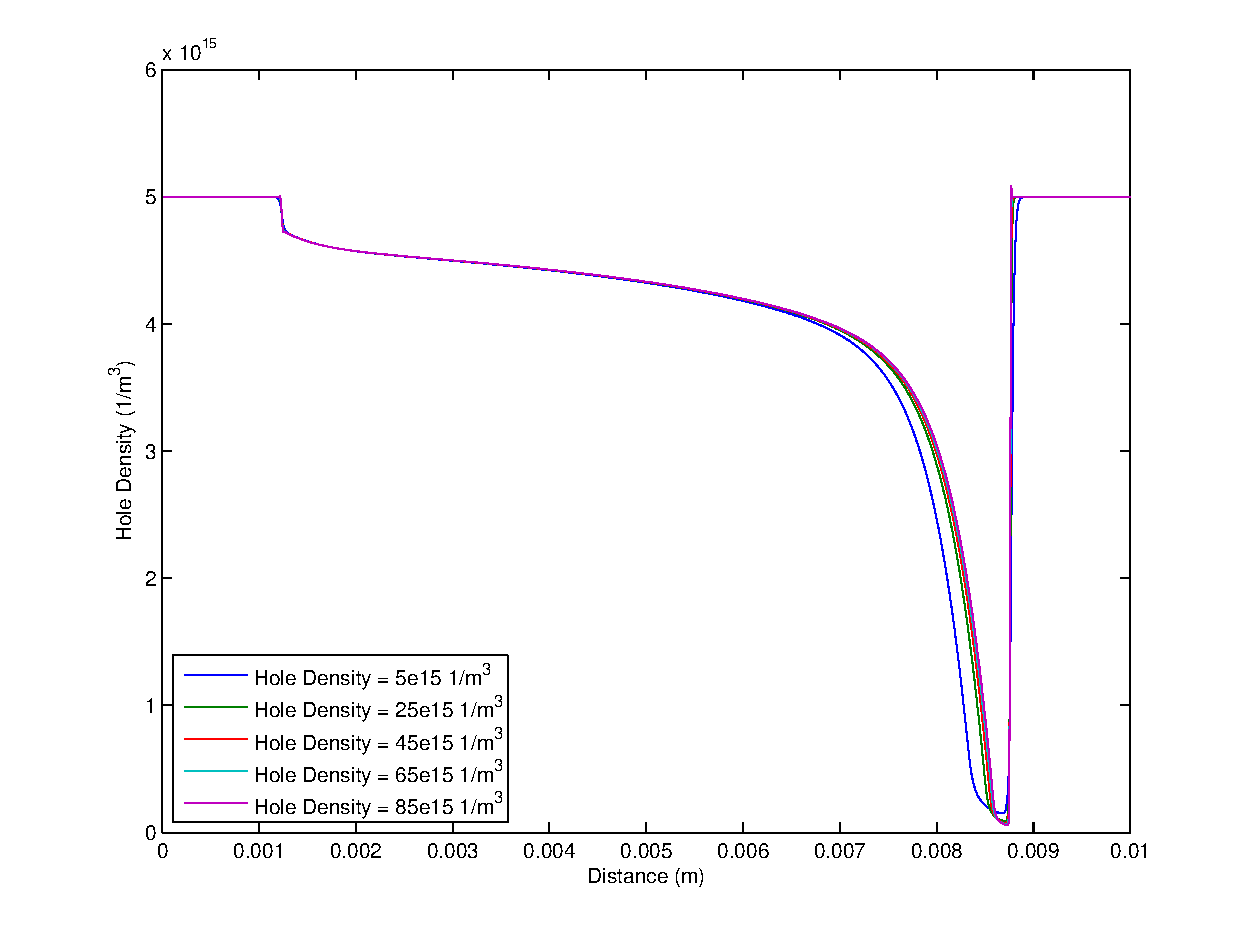
\includegraphics[scale=0.50]{HoleDiff}
\caption{} 
\label{HoleDiff}
\end{figure}

\begin{figure}[!htp]
\centering
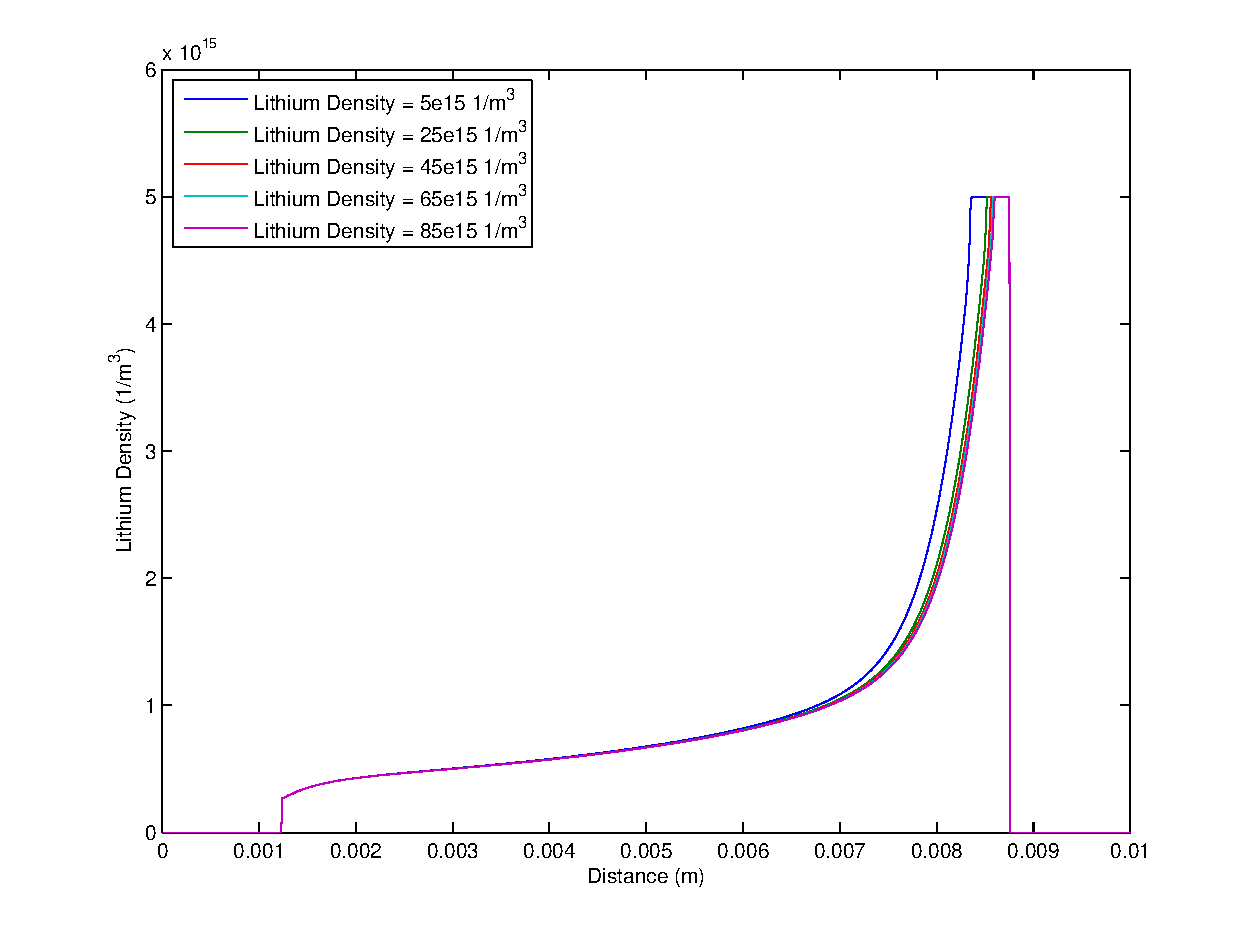
\includegraphics[scale=0.50]{LithiumDiff}
\caption{} 
\label{LithiumDiff}
\end{figure}


\begin{figure}[!htp]
\centering
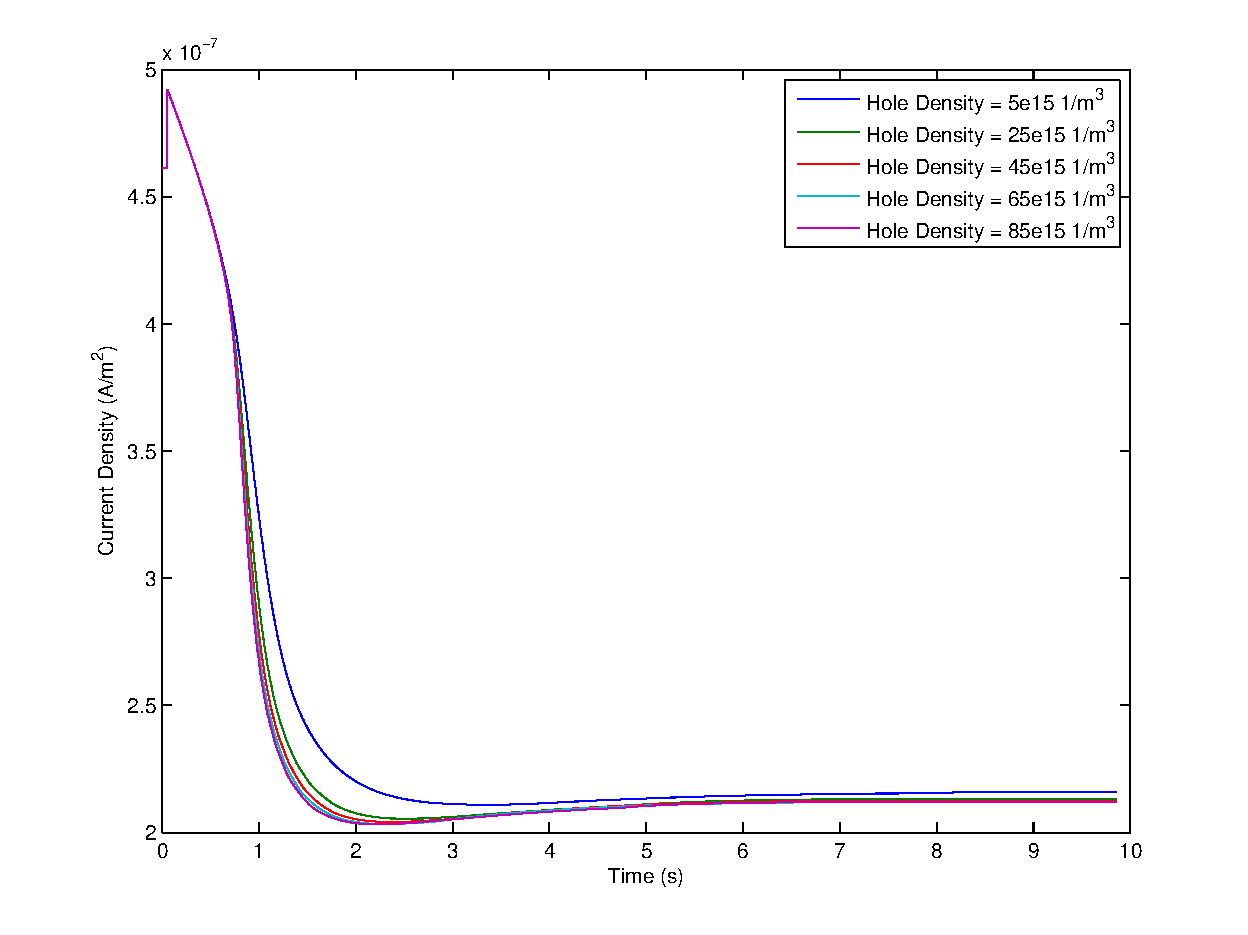
\includegraphics[scale=0.50]{DensityDiff}
\caption{} 
\label{DensityDiff}
\end{figure}

AvDiffn = 100*mean(abs((Jn-J1)/J1))

\begin{figure}[!htp]
\centering
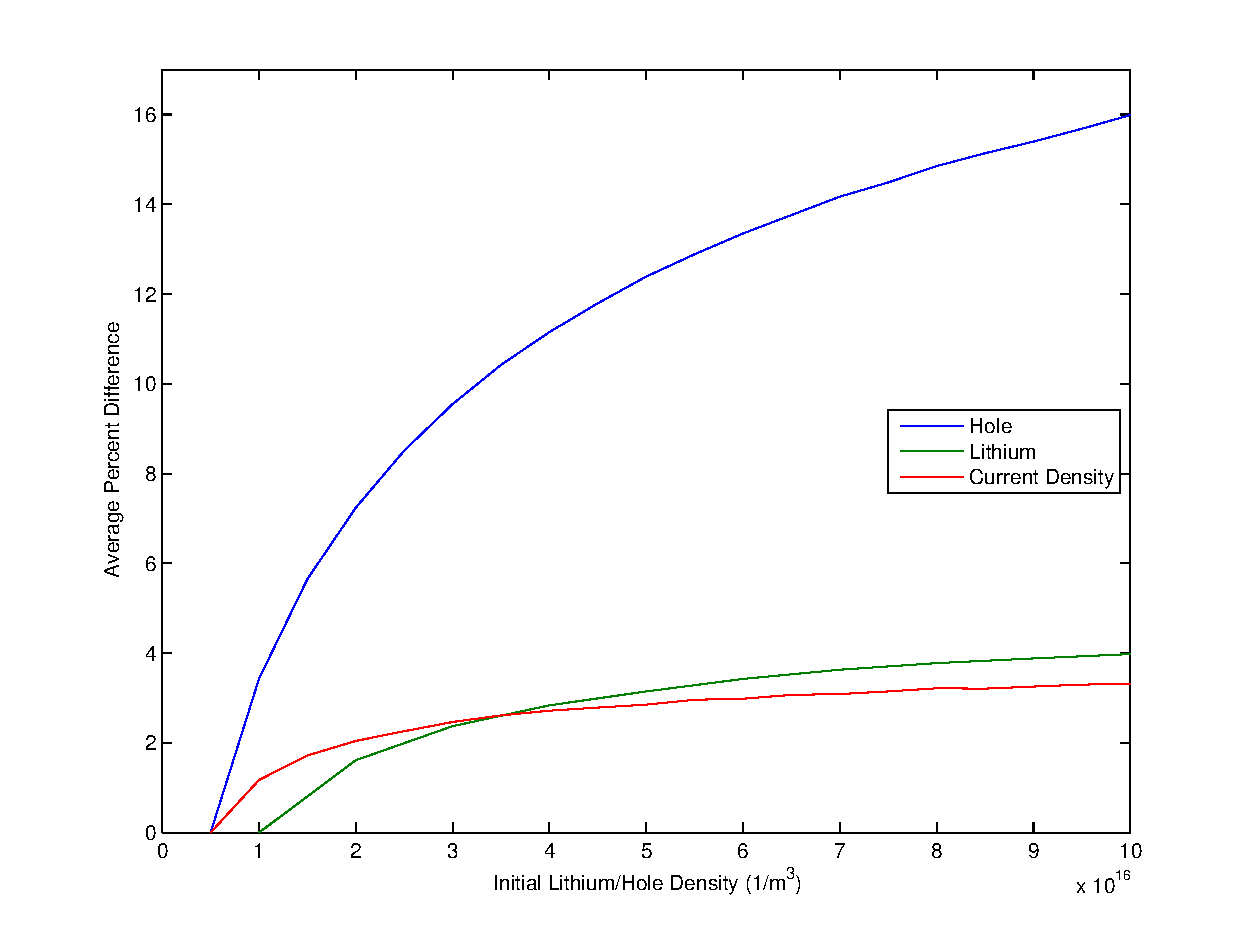
\includegraphics[scale=0.50]{AllDiff}
\caption{} 
\label{}
\end{figure}



\clearpage
\subsection{1-D Memristor Simulation Using a Sinusoid}


Following two figures were created using an AC potential at the contacts. First figure shows (\ref{Bowtie}) shows applied potential versus normalized current. Bow tie plot in this figure is the most commonly seen memristor plot which demonstrates the memory effect of the device since the output current depends on the past states of the device. (add arrows showing the direction of the current on the plot). 
\begin{landscape}
\begin{figure}[!htp]
\centering
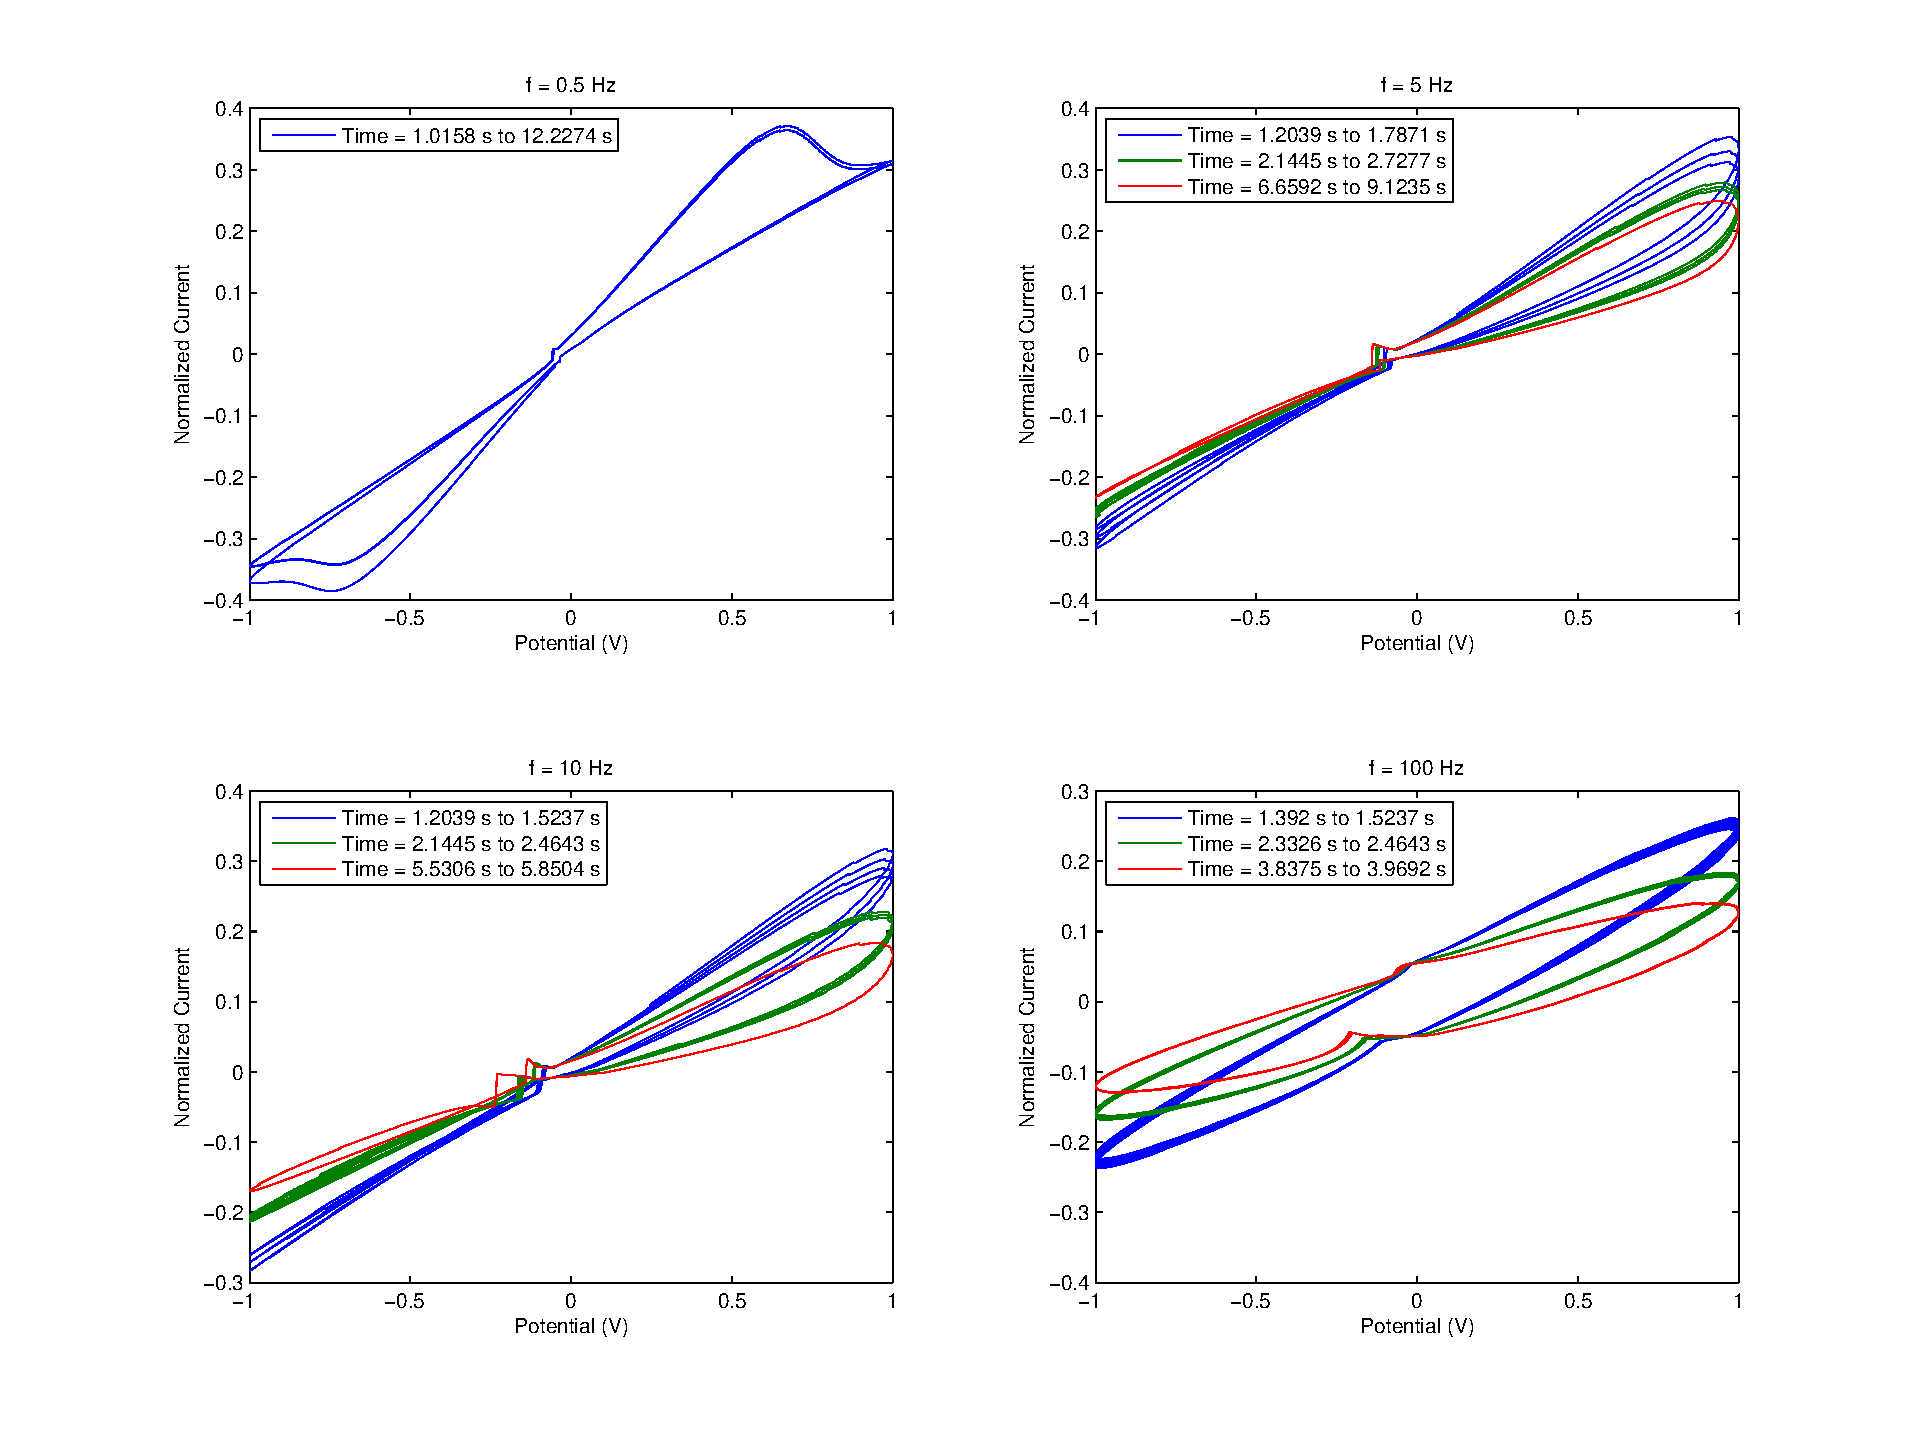
\includegraphics[scale=0.60]{BowtiefAll}
\caption{Normalized Current vs. applied potential at different frequencies} 
\label{Bowtie}
\end{figure}
\end{landscape} 

   
\begin{figure}[!htp]
\centering
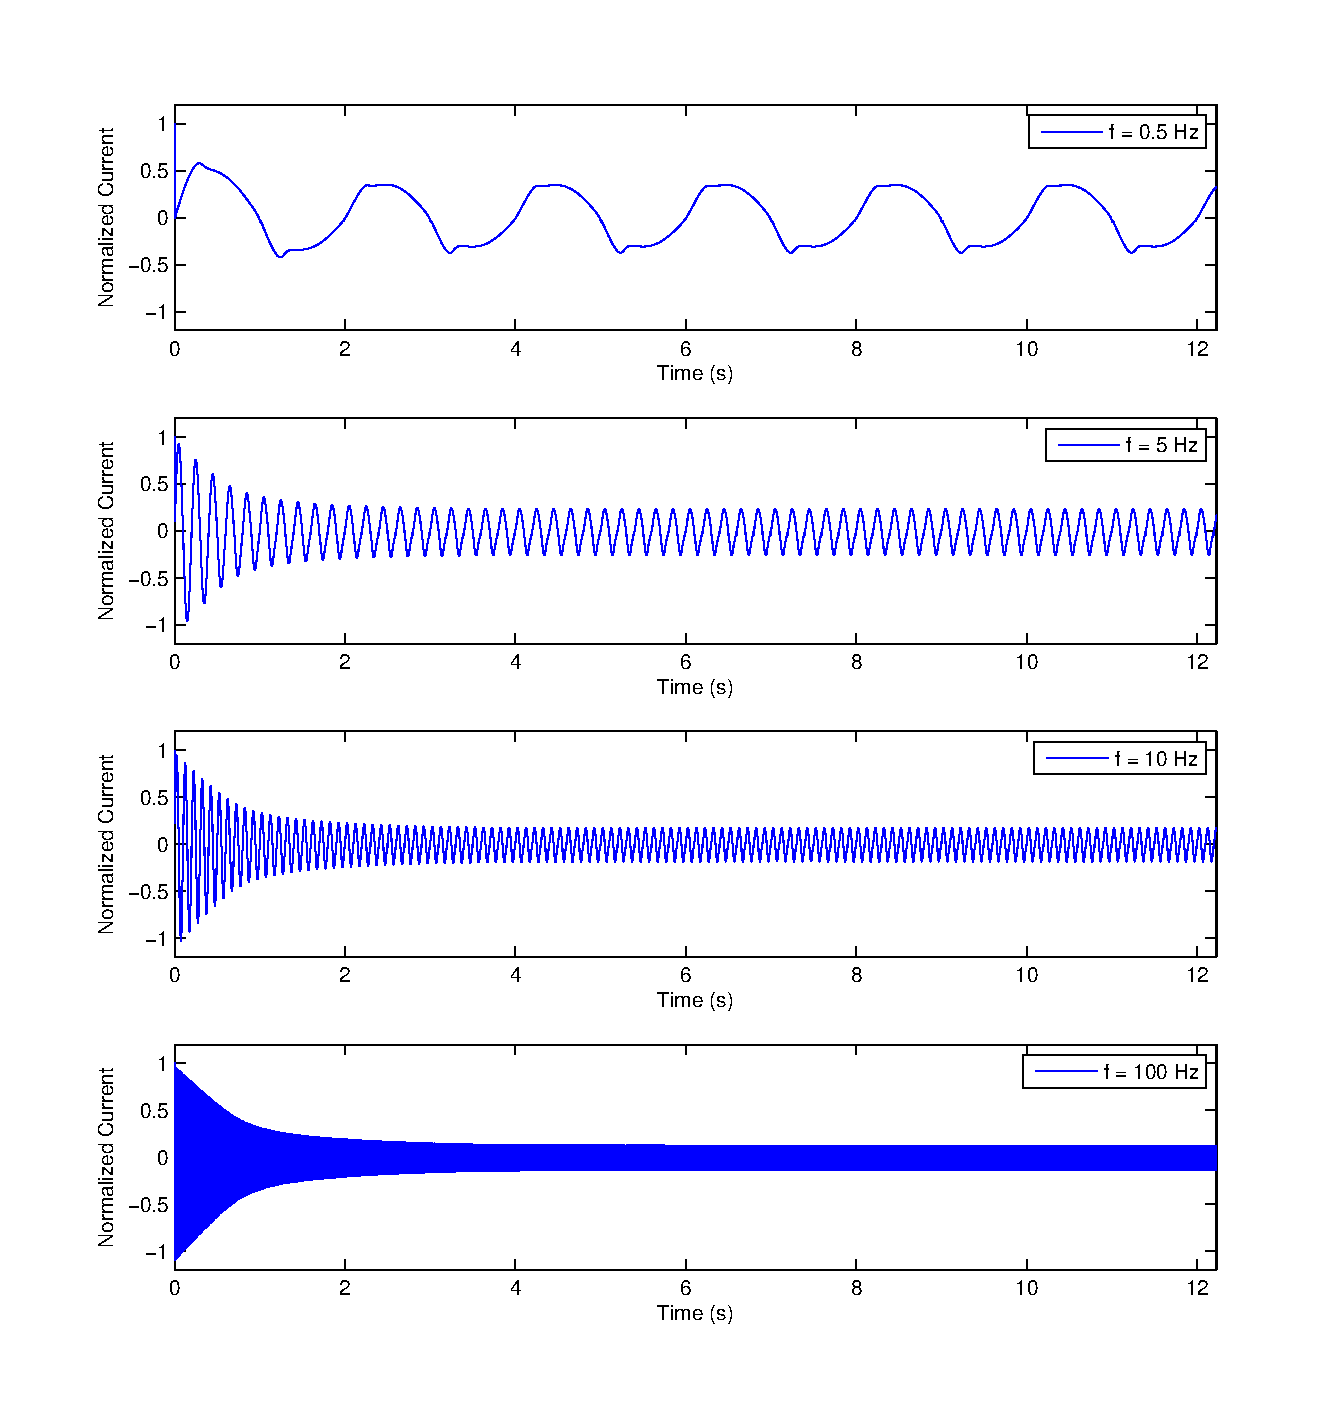
\includegraphics[scale=0.60]{BowtieCurr4f}
\caption{Normalized current over time} 
\label{}
\end{figure}


\begin{landscape}
\begin{figure}[!htp]
\centering
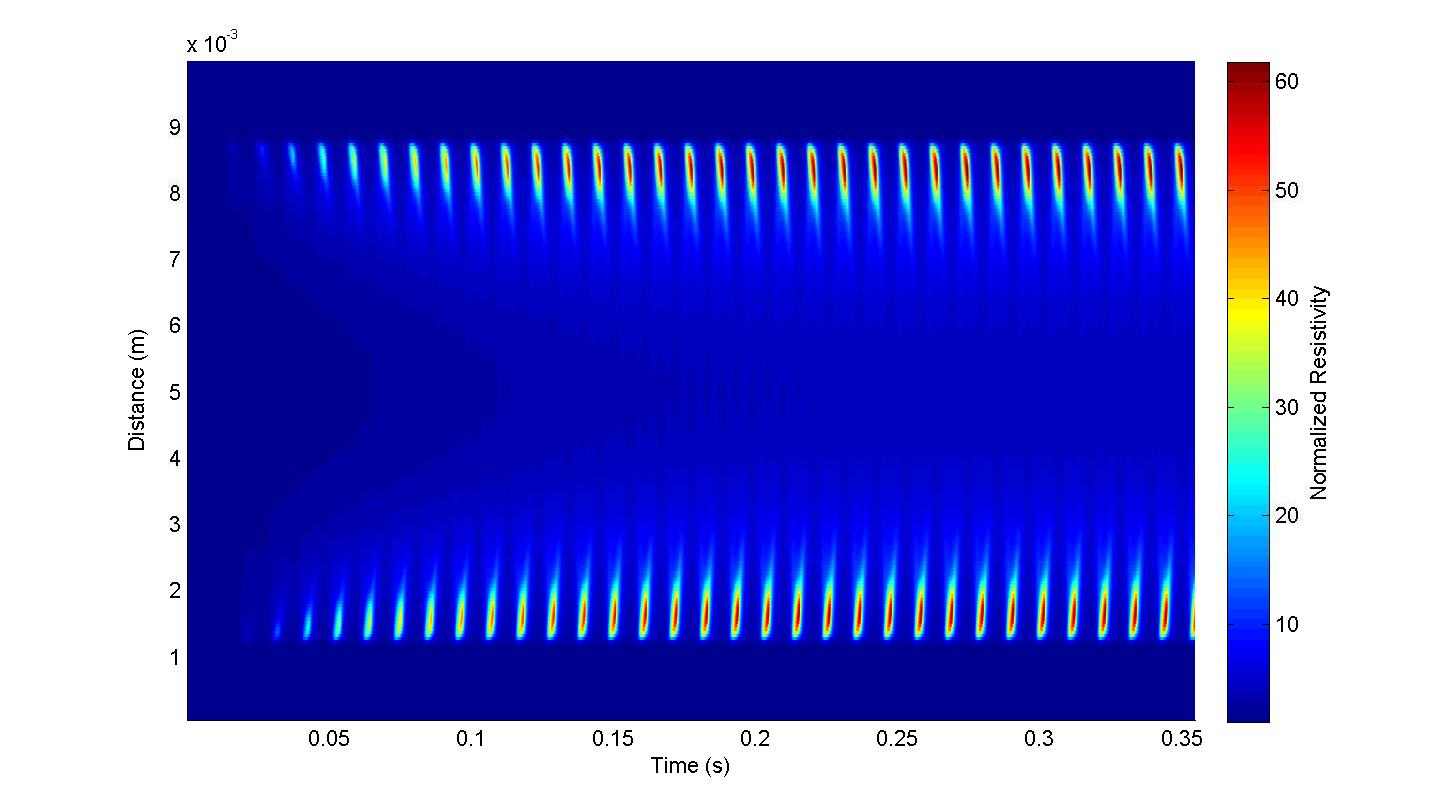
\includegraphics[scale=0.90]{1DMemACResistivity}
\caption{Normalized resistivity over time (f = 5 Hz)} 
\label{}
\end{figure}
\end{landscape} 



\clearpage
\subsection{Changes in Conductivity due to Lithium/Hole Mobility and Applied Potential}

Hopping distance change due to lithium

\begin{figure}[!htp]
\centering
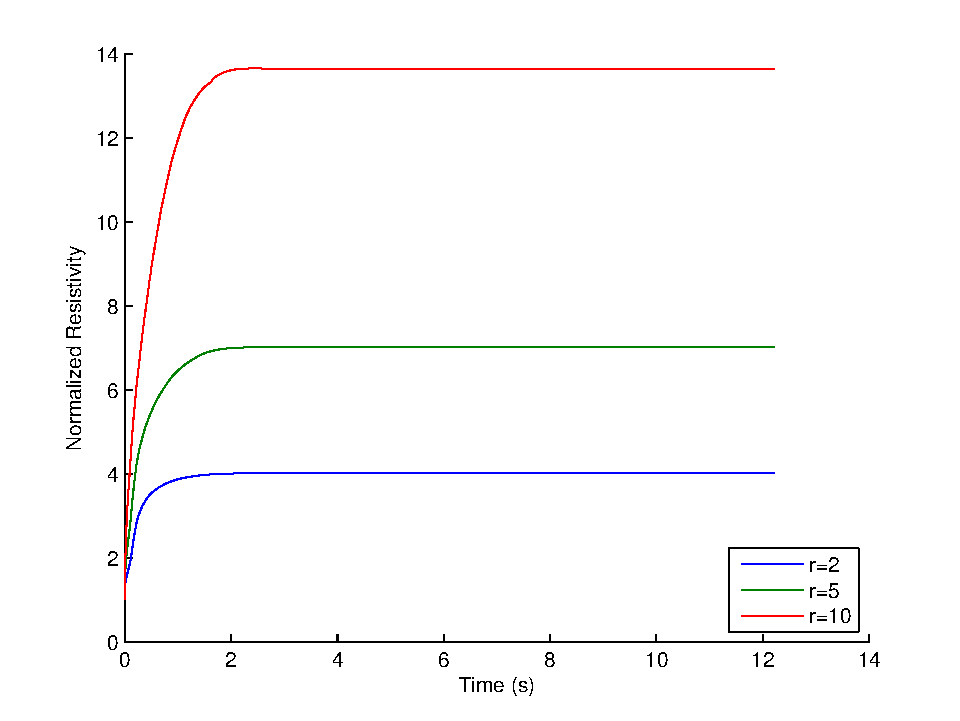
\includegraphics[scale=0.70]{1DHoleMobility}
\caption{} 
\label{}
\end{figure}

Lithium mobility scaling to match experiment
\begin{figure}[!htp]
\centering
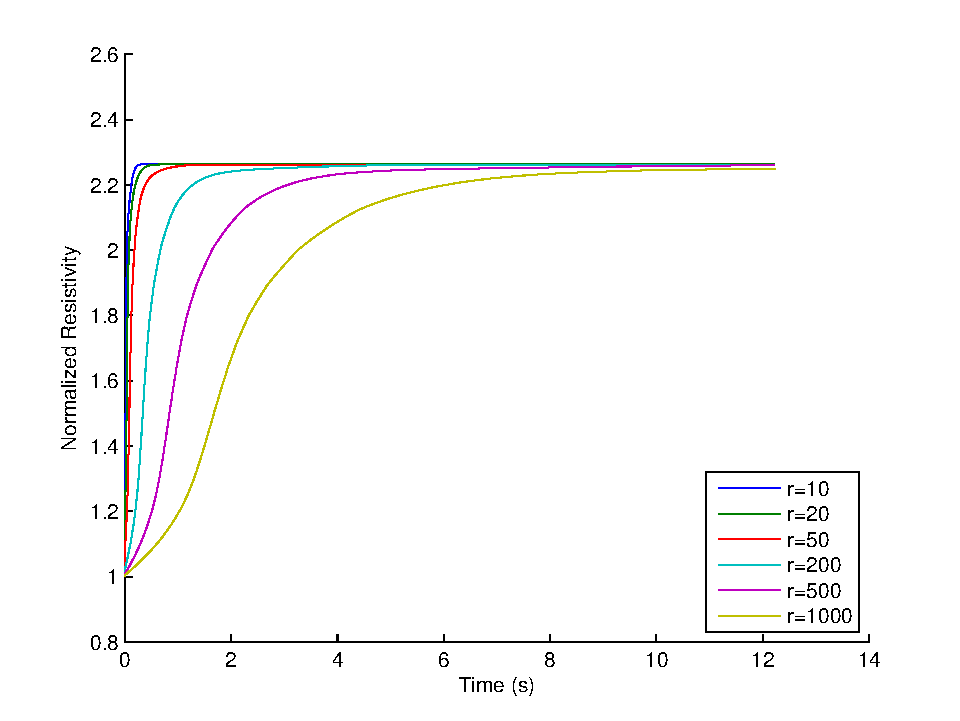
\includegraphics[scale=0.70]{1DLithiumMobility}
\caption{} 
\label{}
\end{figure}

Resistivity change due to applied potential
\begin{figure}[!htp]
\centering
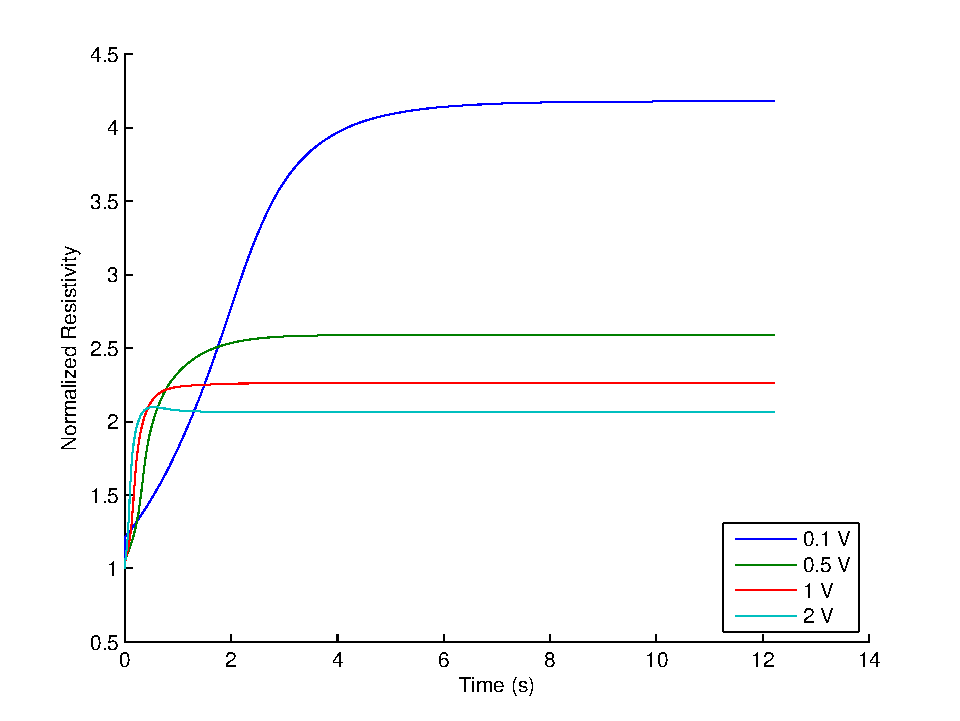
\includegraphics[scale=0.70]{1DMem_V}
\caption{} 
\label{}
\end{figure}

\clearpage
\subsection{Experiment vs. Simulation}